%
% VIT Final Year Project Report.
%
% Author: Santhos Baala RS, VIT University (09MSE038)
%
\documentclass{vitmsprojectreport}

\begin{document}

\makestartingpages
{Using \LaTeX\ for High Quality\\ Project Report Generation}
{Santhos Baala RS}{09MSE038}
{Dr.~Krishna Chandramouli}{Associate Professor}
{Dr.~Sankaran}
{Prof.~Jayaram Reddy A}
{Dr.~Krishna Chandramouli}
{This document describes how to use the vitmsprojectreport class with \LaTeX\ to produce high quality typeset project report that is suitable for submission to the School of Information Technology and Engineering (SITE). The class can further be extended to various courses and department by modifying the title page and department information.}

%======== Contents Start Here ==========%

%----- INTRODUCTION -------%
\chapter{Introduction}

\section{About the Template}

With a basic understanding of the \LaTeX\ language and say 10 to 20 commands, an author can produce beautiful typeset project report quickly, with minimal effort. The purpose of this document is to serve as a user guide for the project report template and document its special behaviours. Examples have also been provided for common tasks such as insertion of images, table, equation, etc., that can be copied as is by the users. It is assumed that the user has a basic knowledge on working of the \LaTeX\ system. Those lacking are strongly urged to lookup some excellent literature through~\cite{kottwitz2011latex}. 

Sufficient examples have been given in the document and as users request solutions for specific problems that they encounter, more will be added. However, an understanding of the \LaTeX\ system will help the user in unexplainable ways\footnote{The \LaTeX\ system is a vast ocean. That said, you can mostly get away with copy-paste skills. You have to observe the source code of the examples and learn}. The main advantage of using the custom class is that, the user need not worry about the final layout. The class may be changed during the development of the project report, the user needs to just place the latest version of the class file, without touching the content\footnote{It is always recommended to get the latest class file from the repository and compile before project report submission.}. \LaTeX, along with the custom class file gives an incredible expressive power its users so that they can focus on the semantics of the document.

\section{Generic \LaTeX\ Commands}

\LaTeX\ contains many commands and with it comes numerous built-in packages that add many features and provide options to customise the output. However, the user is advised to stick to the basic commands, illustrated in this document so that unexpected or incorrect output can be avoided. If, however a specific feature is requested it shall be considered and incorporated into the template. The class file for project report has been extended from the standard \emph{report} class, supplied by \LaTeX. Therefore, whatever applied for report also applies for the custom class file.

\section{Generating the Final Document}

The template development is an ongoing process. It is mature at this point from the point of view of semantics. Layout or default contents (e.g bonafide, acknowledgement, etc.,) may change at a later point in time. Therefore, before generating the final document, please make sure to check out a frozen version of the class file from the repository before compiling the class file.

\section{Asking Questions}

You can post your questions in the forum or if you encounter any problem related to unexpected/incorrect output due to the template send an e-mail to the contributors at the github page.

\section{Contributing}

The project is hosted on GitHub~\cite{github2014} and uses the GIT repository management system. Contributors can fork the project and send pull requests to the repository for the changes to be merged. The patch will be evaluated and if found to be good, merged into the master branch of the repository. If however, a separate template is required for other departments and courses, the project can be forked and maintained separately. Issues, pertaining to the template, such as rendering faults, can be posted in the issues section of the repo. The contributors shall also put up a list of items that need improvement or new features in progress that people can contribute to.

%----- Auto-Generated Pages -------%
\chapter{Auto-Generated Pages}

The parts of the document, unique to the project report are generated by a predefined template, using simple commands. The order in which the commands are issued determine the corresponding order of these individual pages. The arguments that need to be passed to these commands are explained in the following sections. The sequence of commands to generate such pages have already been placed in the example document and it is recommended not to touch those, expect when inserting your project specific information.

\section{The Title Page}

The user can generate the title page using the \verb+\maketitlepage+ command. The detailed syntax is given in \figurename~\ref{fig:maketitlepage_syntax}.

\begin{figure}[htb]
\centering
\hrulefill
\begin{verbatim}
\maketitlepage
{Project Title}
{Name}
{RegNo}
{Guide Name}
{Guide Title} 
\end{verbatim}
\hrulefill
\caption{The syntax of \textbackslash maketitlepage command}
\label{fig:maketitlepage_syntax}
\end{figure}

Note that you should always set the title page to be the first page of the document, so issue this command right after the document begins. The template also collects information like your name and regno when you declare the title page so that it can be auto-inserted into other pages like declaration and bonafide. The following subsections d

\subsection{Project Title}

Your project title should be placed here. If your title is long and you are not satisfied with the way the lines break, use \textbackslash\textbackslash\ to insert line breaks at suitable locations. Note the inclusion of blank space after the backslashes.\\ E.g. \verb+{A very very\\ long long title}+.

\subsection{Regno}

Supply your register number here. A long name will automatically push the register number to the next line. However, to be safe, prepend your RegNo with \textbackslash\textbackslash.\\ E.g. \verb+{\\09MSE038}+.

\subsection{Guide Name}
\label{subsec:guide_name}

Your guide's name goes here. Make sure to add your guide's title too, Prof., Dr., etc. Also, be sure to add a non-breaking space ``$\sim$'' after the title so that unintended line breaks are prevented. Follow the regular convention of first name, last name.\\ E.g. \verb+{Prof.~Robert}+ or \verb+{Dr.~John}+.

\subsection{Guide Title}

Your Guide's title(designation) goes here. Do not abbreviate anything.\\ E.g \verb+{Assistant Professor (Senior)}+.

\section{Declartion Page}

Use \verb+\makedeclarationpage+ command, rest is automatically generated!

\section{Bonafide Page}

Use \verb+\makebonafidepage+ command, rest is automatically generated!

\section{Acknowledgement Page}

Use \verb+\makeackpage+ command to generate the page. The generated text is more than sufficient for acknowledgement. However, if there is a request for custom writeup for the acknowledgement page, we'll consider that\footnote{We don't want to kill creativity!}. There are three arguments to this page as given in \figurename~\ref{fig:makeackpage_syntax}. Make sure to prepend the names with appropriate titles, Mr, Dr, etc., and remember to give a non-breaking space character just after the title as you did for your guide's name in~\ref{subsec:guide_name}

\begin{figure}[htb]
\centering
\hrulefill
\begin{verbatim}
\makeackpage
{Dean Name}
{Program Manager Name}
{Year Co-Ordinator Name}
\end{verbatim}
\hrulefill
\caption{The syntax of \textbackslash makeackpage command.}
\label{fig:makeackpage_syntax}
\end{figure}

\section{Executive Summary Page}

The command \verb+\makeexecsummarypage+ creates the executive summary page. The only argument to this function is your executive summary. Keep it down to 1-2 paragraphs. An example is given in \figurename~\ref{fig:makeexecsummarypage_sample}.

\begin{figure}[htb]
\centering
\hrulefill
\begin{verbatim}
\makeexecsummarypage{
This document describes how to use the vitmsprojectreport
class with \LaTeX\ to produce high quality typeset project
report that is suitable for submission to the School of 
Information Technology and Engineering (SITE). The class 
can further be extended to various courses and department 
by modifying the title page and department information.
}
\end{verbatim}
\hrulefill
\caption{Example usage of the \textbackslash makeexecsummarypage command.}
\label{fig:makeexecsummarypage_sample}
\end{figure}

%------- Text Elements -------%
\chapter{Text Elements}

The chapters, sections and subsections in the document are created with the standard commands \verb+\chapter+, \verb+\section+ and \verb+\subsection+ respectively. The text sections are automatically numbered using arabic numerals and also added to the table of contents. You can create a deeper level using \verb+\subsubsection+. It is recommended to keep the depth restricted to the subsection level. The template doesn't guarantee proper output for beyond that. The following sections illustrate on creating various text structures in the document and cross-references.

\section{Chapters, Sections and Sub-Sections}

Chapters are created with the \verb+\chapter+ command. The chapter title is passed as an argument. Each chapter is automatically placed in a separate page. Sections and Sub-Sections under a chapter are created with the \verb+\section+ and \verb+\subsection+ respectively. The syntax of all the commands are given in \figurename~\ref{fig:text_structure_syntax}.

\begin{figure}[htb]
\centering
\hrulefill
\begin{verbatim}
\chapter{The Chapter Title}
\section{The Section Title}
\subsection{The Sub-Section Title} 
\end{verbatim}
\hrulefill
\caption{Commands to create text structures.}
\label{fig:text_structure_syntax}
\end{figure}

If you want to place a section inside a chapter, place it under that chapter. Similarly, a sub-section meant to be placed inside a section is placed under the corresponding section. That's how levels are created. The sequence of commands in \figurename~\ref{fig:text_structure_syntax} will create a sub-section, under a section, which in turn is under a chapter.

\section{Lists}

List is inherited directly from vanilla \LaTeX\ list. You can look them up from any tutorial for \LaTeX lists, preferably from~\cite{kottwitz2011latex}. We give a short example of an unordered list and an ordered list over here. Changing the list style, bullet shape, etc., is your choice. \emph{Note that an empty list(list with no items) will throw an error during compilation.} More information on the list structure is available at \url{http://en.wikibooks.org/wiki/LaTeX/List_Structures#Enumerate}.

\subsection{Unordered}
An unordered list is generated by the \verb+\begin{itemize}...\end{itemize}+ environment with \verb+\item+ commands inside. The listing in \figurename~\ref{fig:itemize_sample} generates an unordered list, placed to the right of the same figure.

\begin{figure}[htb]
\centering
\hrulefill
%Source Code
\begin{verbatim}
\begin{itemize}
\item C
\item C++
\item Java
\end{itemize}
\end{verbatim}

\vspace{-2.65cm}
\hspace{5cm}
\begin{minipage}[r][2.75cm][l]{5cm}
%Output
\begin{itemize}
\item C
\item C++
\item Java
\end{itemize}
\end{minipage}

\hrulefill
\caption{Unordered list example.}
\label{fig:itemize_sample}
\end{figure}

\subsection{Ordered}

Ordered lists can be generated by the \verb+\begin{enumeration}...\end{enumeration}+ environment with \verb+\item+ commands inside. The listing in \figurename~\ref{fig:enumerate_sample} generates an orders list, placed to the right of the same figure.

\begin{figure}[htb]
\centering
\hrulefill
%Source Code
\begin{verbatim}
\begin{enumerate}
\item C 
\item C++ 
\item Java
\end{enumerate}
\end{verbatim}

\vspace{-2.65cm}
\hspace{5cm}
\begin{minipage}[r][2.75cm][l]{5cm}
%Output
\begin{enumerate}
\item C
\item C++
\item Java 
\end{enumerate}
\end{minipage}

\hrulefill
\caption{Ordered list example.}
\label{fig:enumerate_sample}
\end{figure}

The default numbering scheme of the template is arabic and it is recommended not to change that. The numbering scheme for nested ordered lists is automatically managed.

\subsection{Description List}

Sometimes, it is required to render something like a definition list. Although semantically it isn't a list, it follows the same syntax structure. Such special type of lists can be created with the \verb+\begin{description}...\end{description}+ environment and the \verb+\item[...]+ command. The usage of one such special list is illustrated in \figurename~\ref{fig:description_list_sample} along with the output.

\begin{figure}[htb]
\centering
\hrulefill
%Source Code
\begin{verbatim}
\begin{description}
\item[C] The first item's description
\item[C++] The second item's description
\item[Java] The third item's description
\end{description}
\end{verbatim}

\vspace{0.5cm}
\begin{minipage}[l][2.75cm][l]{\columnwidth}
%Output
\begin{description}
\item[C] The first item's description
\item[C++] The second item's description
\item[Java] The third item's description
\end{description}
\end{minipage}

\hrulefill
\caption{Description list example.}
\label{fig:description_list_sample}
\end{figure}

\section{Footnotes}

A footnote is an ancillary piece of information, something that is additional but less important. They are placed at the bottom of the page\footnote{This is a sample footnote}. The template automatically adds a horizontal rule to separate it from the main flow of the document. Each footnote is numbered, specific to the page in which it resides. A footnote is added through the \verb+\footnote+ command, with the actual contents of the footnote as the argument. Footnotes are meant to be added along the regular flow of the document. It is illustrated by \figurename~\ref{fig:footnote_sample}.

\begin{figure}[htb]
\centering
\hrulefill
\begin{verbatim}
This is the regular flow of document\footnote{This piece of 
text is treated as a footnote}.
\end{verbatim}
\hrulefill
\caption{An example footnote.}
\label{fig:footnote_sample}
\end{figure}

There may be multiple pages in the same page. If the placement of the footnote flows into the next page, it is automatically managed.

\section{Cross-References}

Other elements in the document can be referenced via the \verb+\ref+ command at the location where a reference is to be inserted and the target identifies itself with a \verb+\label+ command. 

\section{External References}

TODO

%------- Floating Structures -------%
\chapter{Floating Structures}

Elements that are embedded in a text document are termed as floating structures. These include figures, tables, equations, algorithms, etc. In the following sections, examples have been provided on how to use these elements and how the template behaviour can be controlled through the various options available.

\section{Figures}

Figures are handled in the standard \LaTeX\ manner. An minimalistic example is given in \figurename~\ref{fig:figure_sample}.

\begin{figure}[htb]
\centering
\hrulefill
\begin{verbatim}
\begin{figure}[htb]
\centering
\includegraphics[width=2.5in]{myfigure}
\caption{My figure caption.}
\label{fig:identify_the_figure}
\end{figure}
\end{verbatim}
\hrulefill
\caption{Embedding a figure.}
\label{fig:figure_sample}
\end{figure}

The figure is placed inside the \verb+\begin{figure}...\end{figure}+ environment. The options passed to the environment is the figure placement priority preference, h - at the current location, t - top and b - bottom. \verb+\centering+ indicates that the figure and caption should be placed at the centre. \verb+\includegraphics+ is self explanatory, with the width option and the source file. Note that the source file does not specify the file extension, we let \LaTeX\ choose the best available format automatically.

A few examples of figures have been put up here. Check the source tex of this document to understand more.

\begin{figure}[t]
\centering
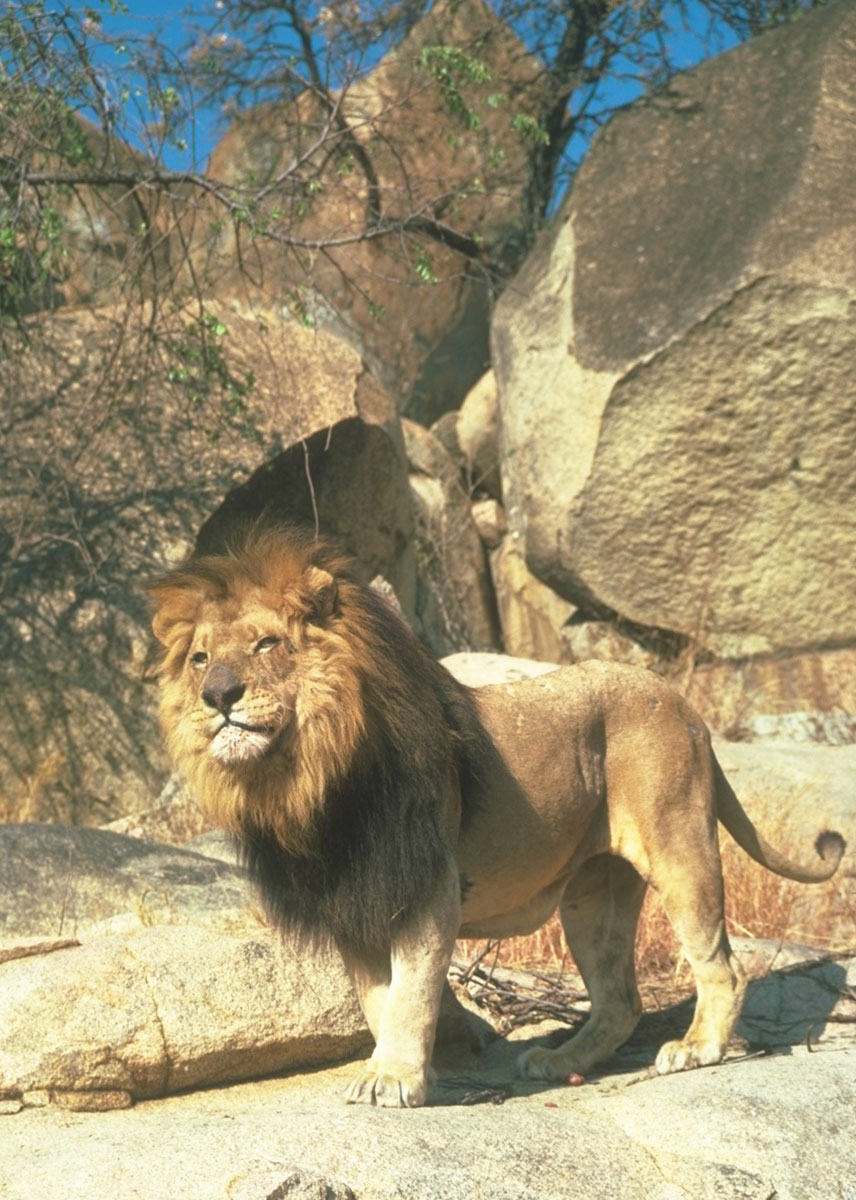
\includegraphics[width=0.5\textwidth]{105003.jpg}
\caption{Framework overview}
\label{fig:framework}
\end{figure}

\section{Tables}

\section{Algorithms}

\chapter{Equations}

%====== Auto-Insert Chapter for References =======
\insertreferences{Example}
%=================================================

\end{document}